\documentclass[compress]{beamer}
\usepackage{ifthen,verbatim}

\newcommand{\isnote}{}
\xdefinecolor{lightyellow}{rgb}{1.,1.,0.25}
\xdefinecolor{darkblue}{rgb}{0.1,0.1,0.7}
\xdefinecolor{darkgreen}{rgb}{0.,0.3,0.}

%% Uncomment this to get annotations
%% \def\notes{\addtocounter{page}{-1}
%%            \renewcommand{\isnote}{*}
%% 	   \beamertemplateshadingbackground{lightyellow}{white}
%%            \begin{frame}
%%            \frametitle{Notes for the previous page (page \insertpagenumber)}
%%            \itemize}
%% \def\endnotes{\enditemize
%% 	      \end{frame}
%%               \beamertemplateshadingbackground{white}{white}
%%               \renewcommand{\isnote}{}}

%% Uncomment this to not get annotations
\def\notes{\comment}
\def\endnotes{\endcomment}

\setbeamertemplate{navigation symbols}{}
\setbeamertemplate{headline}{\mbox{ } \hfill
\begin{minipage}{5.5 cm}
\vspace{-0.75 cm} \small
\end{minipage} \hfill
\begin{minipage}{4.5 cm}
\vspace{-0.75 cm} \small
\begin{flushright}
\ifthenelse{\equal{\insertpagenumber}{1}}{}{Jim Pivarski \hspace{0.2 cm} \insertpagenumber\isnote/\pageref{numpages}}
\end{flushright}
\end{minipage}\mbox{\hspace{0.2 cm}}\includegraphics[height=1 cm]{../cmslogo} \hspace{0.1 cm} \includegraphics[height=1 cm]{../tamulogo} \hspace{0.01 cm} \vspace{-1.05 cm}}

\newcommand{\s}[1]{{\mbox{\scriptsize #1}}}

\begin{document}
\begin{frame}
\vfill
\begin{center}
\textcolor{darkblue}{\Large Track-Based Alignment Status and Outlook}

\vfill
\begin{columns}
\column{0.3\linewidth}
\begin{center}
\large
Jim Pivarski
\end{center}
\end{columns}

\begin{columns}
\column{0.3\linewidth}
\begin{center}
\scriptsize
{\it Texas A\&M University}
\end{center}
\end{columns}

\vfill
28 September, 2010

\end{center}
\end{frame}

%% \begin{notes}
%% \item This is the annotated version of my talk.
%% \item If you want the version that I am presenting, download the one
%% labeled ``slides'' on Indico (or just ignore these yellow pages).
%% \item The annotated version is provided for extra detail and a written
%% record of comments that I intend to make orally.
%% \item Yellow notes refer to the content on the {\it previous} page.
%% \item All other slides are identical for the two versions.
%% \end{notes}

\small

\begin{frame}
\frametitle{Outline}
\begin{itemize}\setlength{\itemsep}{0.5 cm}
\item Alignment projections with 20--30~pb$^{-1}$
\item Current issue: variation of residuals within a chamber
\item Upcoming endcap disk improvements
\item Update on track-based vs.\ hardware ``twist''
\item Potential method to resolve the twist
\item Upcoming sign-off schedule (new constants for re-reco)
\end{itemize}
%% \hspace{-0.83 cm} \textcolor{darkblue}{\Large Outline2}
\end{frame}

\begin{frame}
\frametitle{Alignment resolution projections}

\begin{itemize}
\item Below: latest alignment methods, current best understanding, \\
  ``resolution'' = RMS of $x_\s{aligned} - x_\s{true}$ in simulated alignment
\item Collisions muons only: $p_T > 20$~GeV/$c$ (cosmic-ray simulation
  yields 0.3~mm for top and bottom chambers of barrel)
\begin{center}
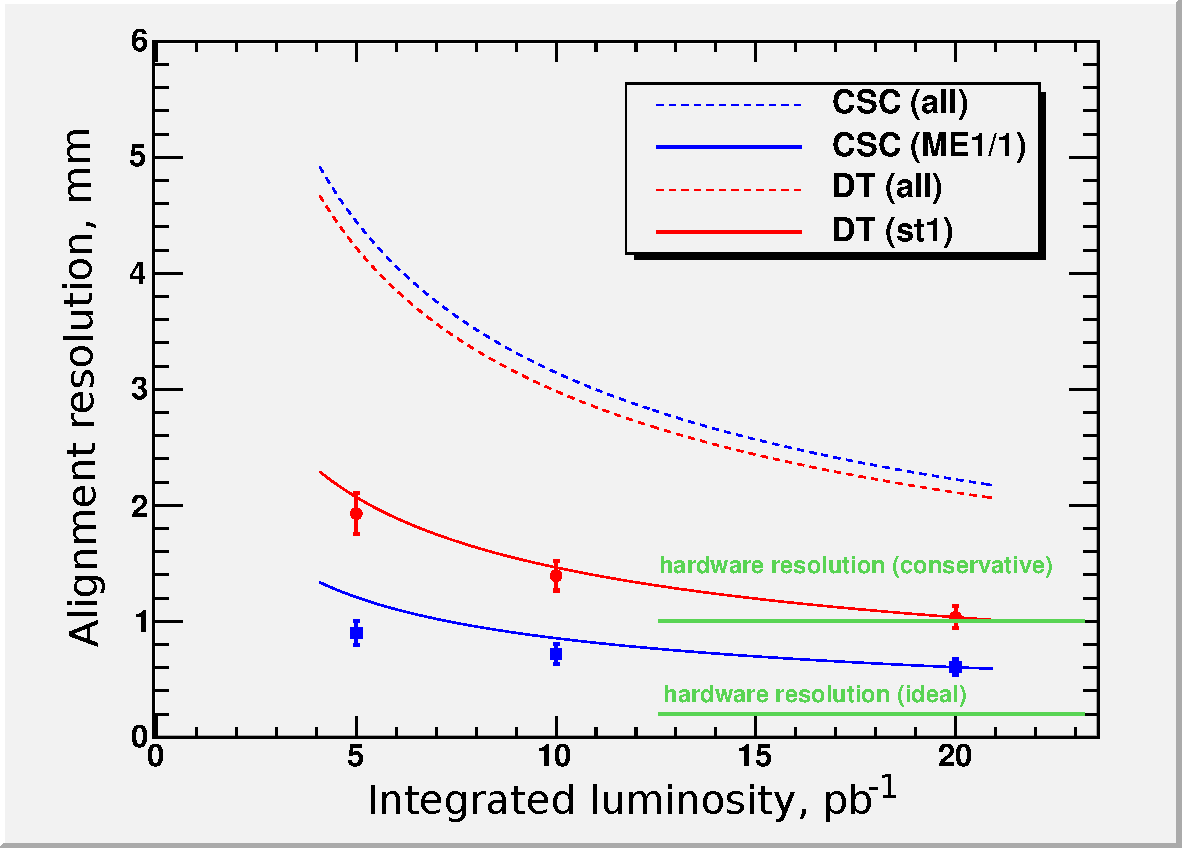
\includegraphics[width=0.65\linewidth]{st1_me11.pdf}
\end{center}
\item Only a significant contribution with ``{\it tens} of pb$^{-1}$'' of \mbox{collisions muons\hspace{-1 cm}}
\end{itemize}
\end{frame}

\begin{frame}
\frametitle{Alignment resolution projections}
\begin{itemize}
\item \textcolor{darkblue}{Question:} ``I remember seeing more optimistic projections \\ at the end of last year--- what happened?''

\textcolor{darkblue}{Answer:} a single bug affected the interpretation
of several studies with low-momentum muons by artificially pinching
the distributions

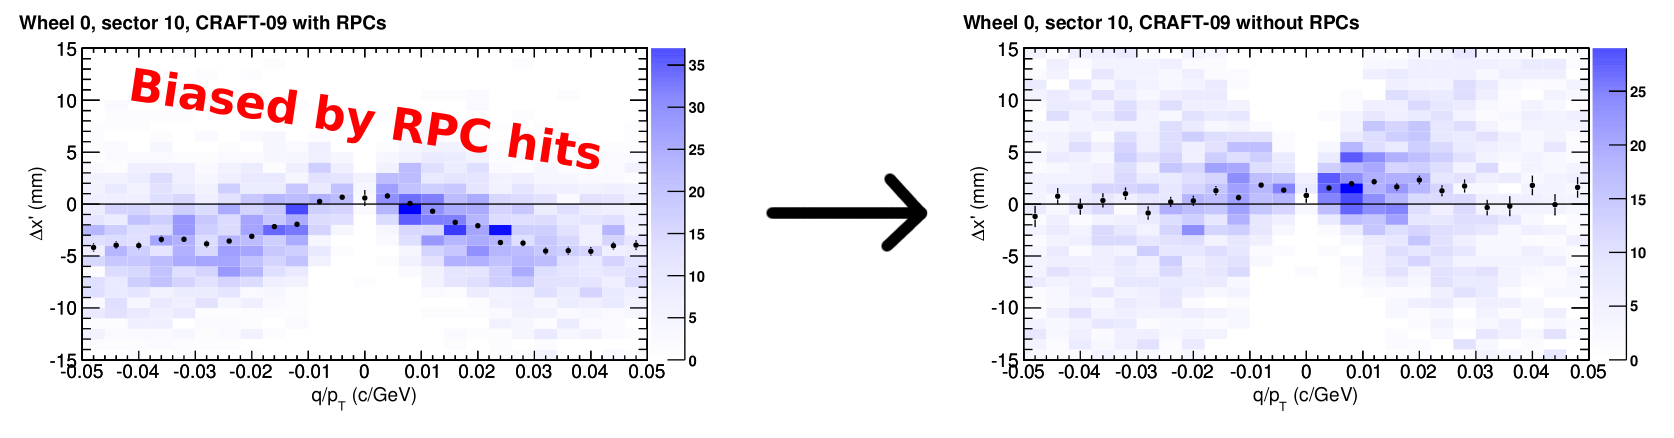
\includegraphics[width=\linewidth]{rpcbiasfix.png}

\hfill 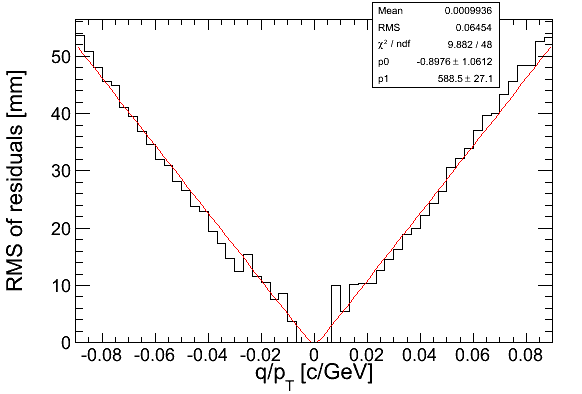
\includegraphics[width=0.5\linewidth]{qoverpt_residualswidth.png}

\vspace{-3.5 cm}
\item Resolving this issue results in \\ residuals distributions
  consistent \\ with Moli\`ere theory and brings \\ resolution
  projections more in line \\ with CSA08 and the ``50~pb$^{-1}$ \\
  simulation'' studies of 2009

\vspace{0.1 cm}
The baseline is ``tens of pb$^{-1}$'', \\ exact value depending on desired resolution
\end{itemize}
\end{frame}

\begin{frame}
\frametitle{Alignment resolution projections}
\begin{itemize}
\item Lowering momentum cuts improve resolution (here: $p_T > 20$~GeV/$c$ $\to$ $p_T > 15$~GeV/$c$)
\item But low-momenta are more susceptible to sources of bias, must be checked in data
\end{itemize}
\begin{center}
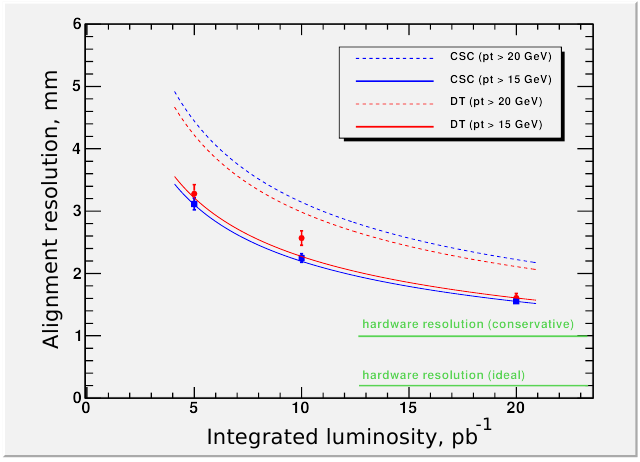
\includegraphics[width=0.75\linewidth]{lowercut.png}
\end{center}
\end{frame}

\begin{frame}
\frametitle{Residuals within a chamber}
\begin{itemize}
\item Standard tool: subdivide residuals distribution into bins
  smaller than the chambers to be sure that sharp changes in residuals
  are only at the chamber borders
\item \textcolor{blue}{Blue ellipse:} example of a discontinuity at a chamber border
\item \textcolor{red}{Red ellipse:} unexpected discontinuity inside of a chamber {\scriptsize (observed in local $y$ residuals, which corresponds to global $z$ (parallel-to-beamline) positions)}
\end{itemize}
\begin{center}
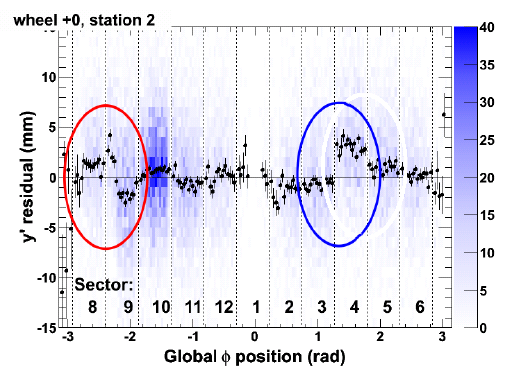
\includegraphics[width=0.65\linewidth]{localyplot.png}
\end{center}
\end{frame}

\begin{frame}
\frametitle{Residuals within a chamber}
\begin{columns}
\column{0.4\linewidth}
\begin{itemize}
\item \mbox{Related to which station~1\hspace{-5 cm}} \\ \mbox{chamber the track went\hspace{-5 cm}} \\ \mbox{through before station~2\hspace{-5 cm}}

\textcolor{red}{red: segment in station~1, sector~8}

\textcolor{blue}{blue: segment in station~1, sector~9}

\textcolor{darkgreen}{green: no segment in either}

\item Checked for:
\begin{itemize}
\item \mbox{track-propagation\hspace{-2 cm}} \\ \mbox{bias from station~1\hspace{-2 cm}}
\item \mbox{bad trigger geometry\hspace{-2 cm}}
\item \mbox{dead groups of wires\hspace{-2 cm}}
\end{itemize}

\mbox{None of the above observed\hspace{-5 cm}}

\item \mbox{(Note: even with wide bins,\hspace{-2 cm}} \\ \mbox{uncertainty in mean local y residual from collisions is $\pm$5~mm (low-$|p|$))\hspace{-15 cm}}
\end{itemize}
\column{0.6\linewidth}
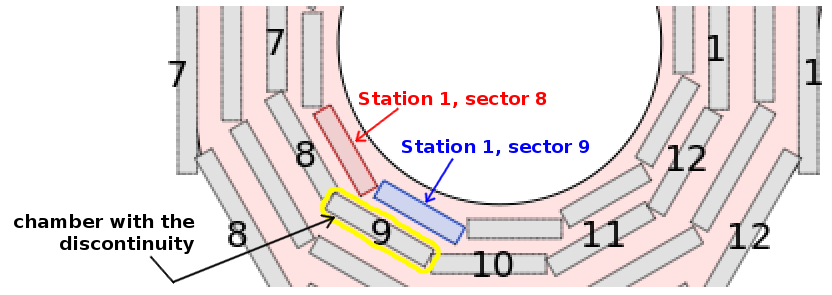
\includegraphics[width=\linewidth]{diagram.png}

\vspace{0.25 cm}
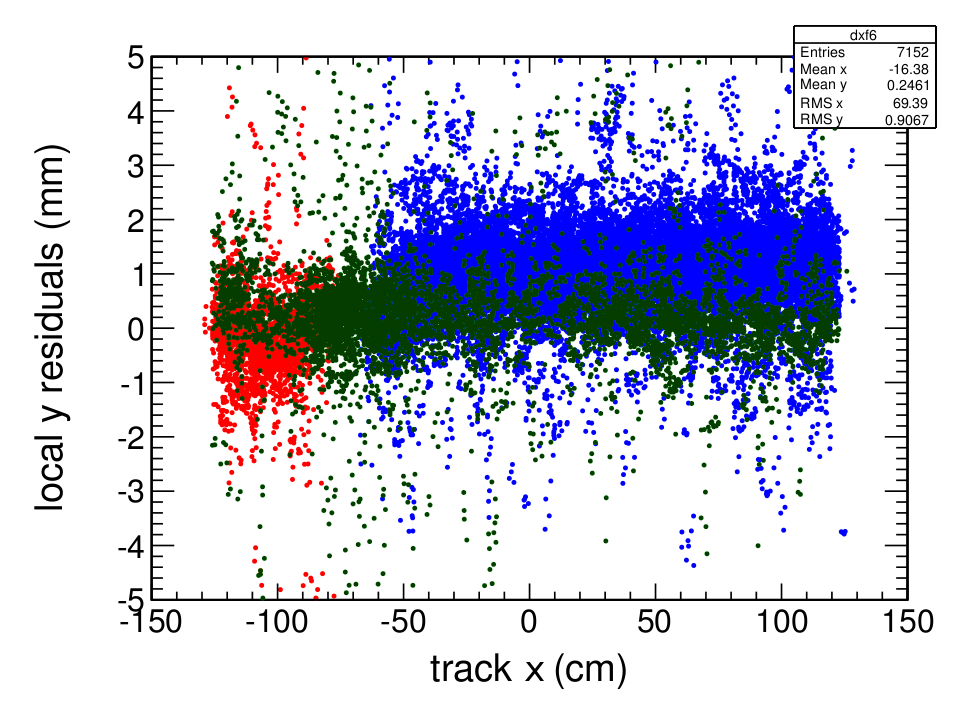
\includegraphics[width=\linewidth]{residuals_in_chamber.png}
\end{columns}
\end{frame}

\begin{frame}
\frametitle{Endcap disk alignment}
\begin{itemize}
\item All track-based alignment procedures will follow this transition:

high-$p_T$ cosmics \hspace{0.1 cm} $\to$ \hspace{0.1 cm} medium-$p_T$ cosmics \hspace{0.1 cm} $\to$ \hspace{0.1 cm} same-$p_T$ collisions

\item We can already step forward in endcap disk alignment (in which whole
  disks are treated as rigid bodies) with some gains in resolution

\item Example disk alignment with cosmics (rigid-body disk $\Rightarrow$ sinusoidal):
\end{itemize}

\vspace{-0.5 cm}
\begin{columns}
\column{0.5\linewidth}
\begin{center}
with $p_T > 100$~GeV/$c$ (current)
\end{center}

\vspace{-0.25 cm}
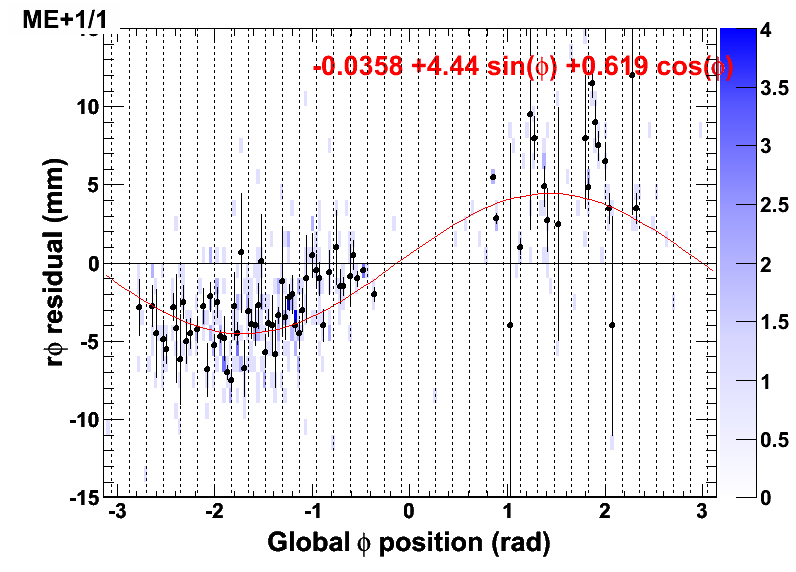
\includegraphics[width=\linewidth]{endcap_highmomentum.png}

\column{0.5\linewidth}
\begin{center}
with $p_T > 10$~GeV/$c$
\end{center}

\vspace{-0.25 cm}
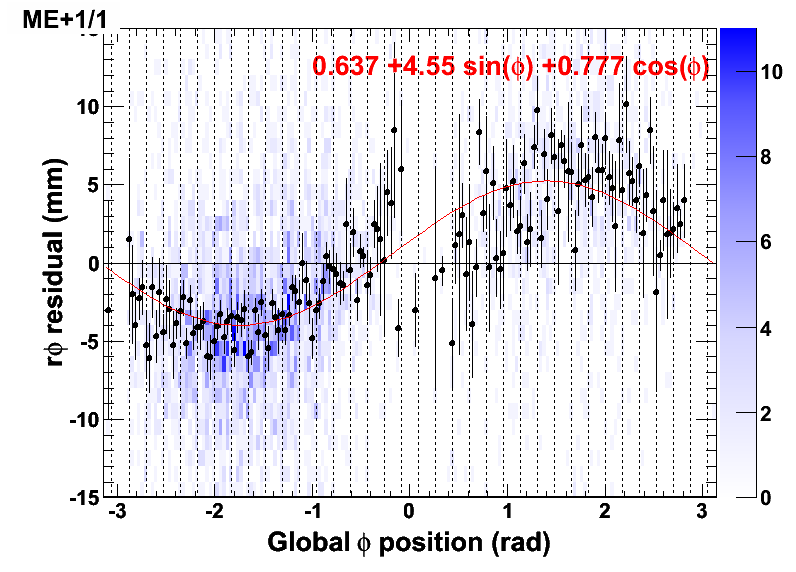
\includegraphics[width=\linewidth]{endcap_allmomenta.png}
\end{columns}

\begin{itemize}
\item Switching to collisions would fill in the $\phi = 0$ and $\pi$ regions
\end{itemize}
\end{frame}

\begin{frame}
\frametitle{Track-based vs.\ hardware ``twist''}
\begin{columns}
\column{0.5\linewidth}
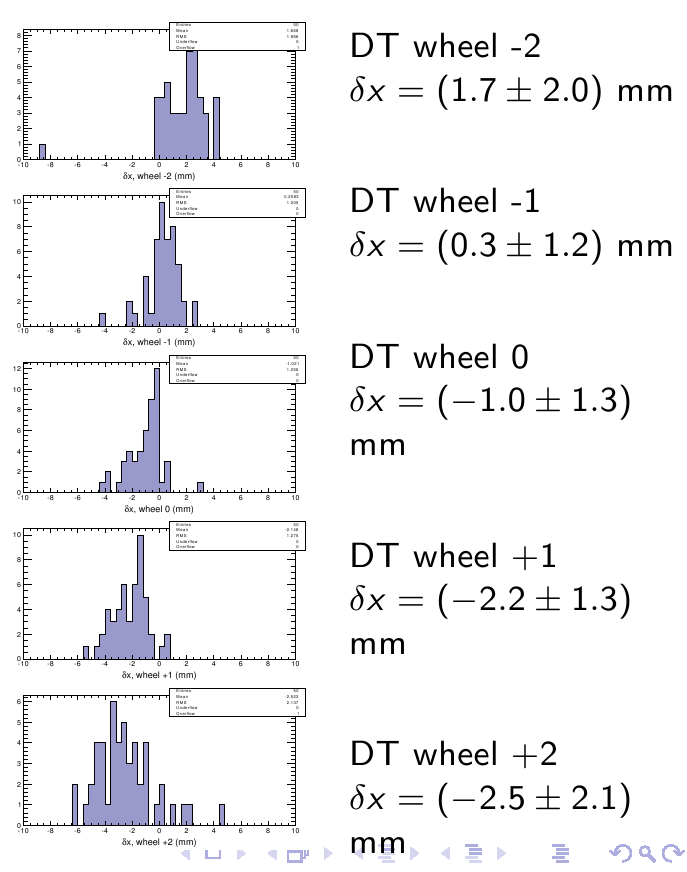
\includegraphics[width=\linewidth]{twist1.png}

\column{0.5\linewidth}
\begin{itemize}
\item \textcolor{darkblue}{Reminder:} primary difference between
  barrel track-based and hardware geometries is a twist of one
  relative to the other

\item Plots on left: track-based minus hardware by wheel

\item Effect on \\ track \\ curvatures \\ (versus $\eta$):

\vspace{-1.9 cm}
\hfill 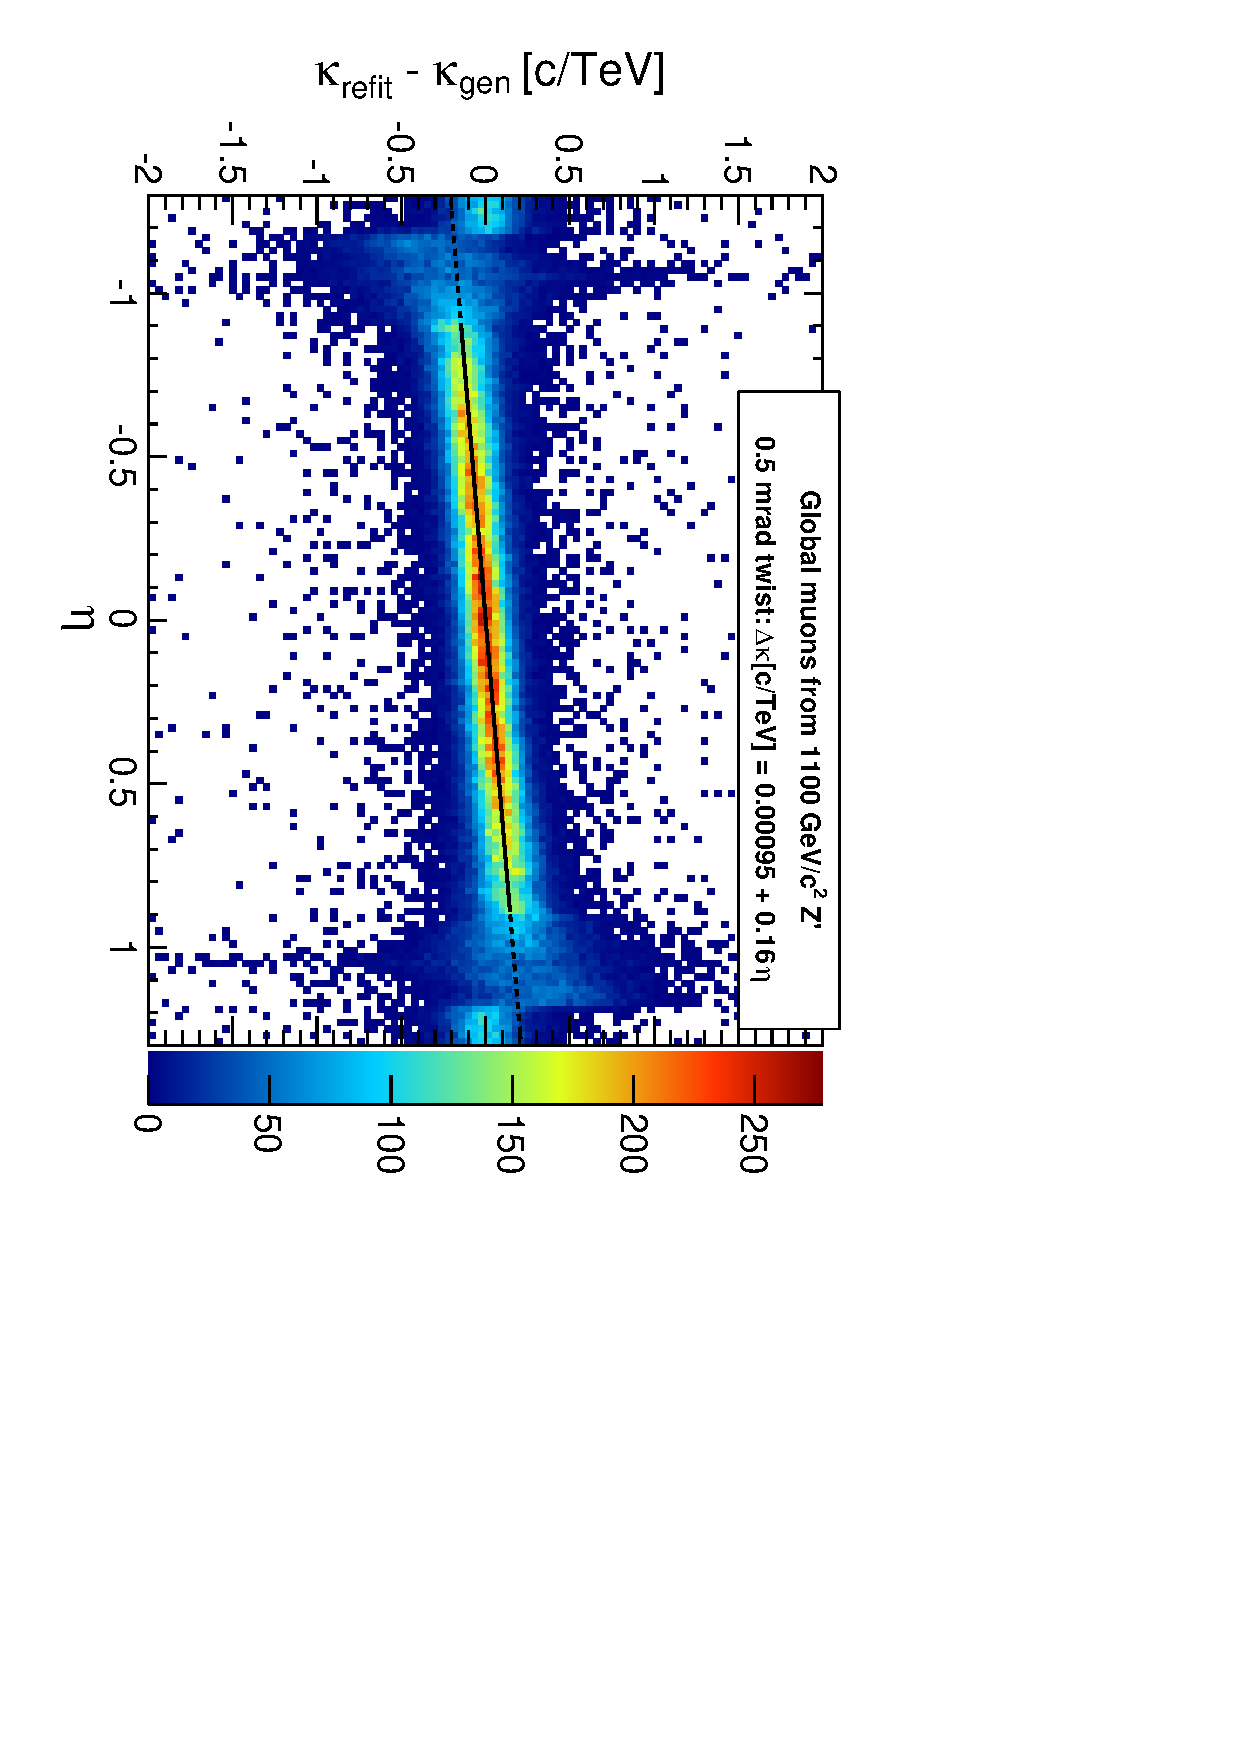
\includegraphics[height=0.65\linewidth, angle=90]{curvbias_vseta_twist0_5mrad_1100_GlobalMuons2.pdf}

\item Effect on \\ $Z'$ mass \\ resolution:

\vspace{-1.3 cm}
\hfill 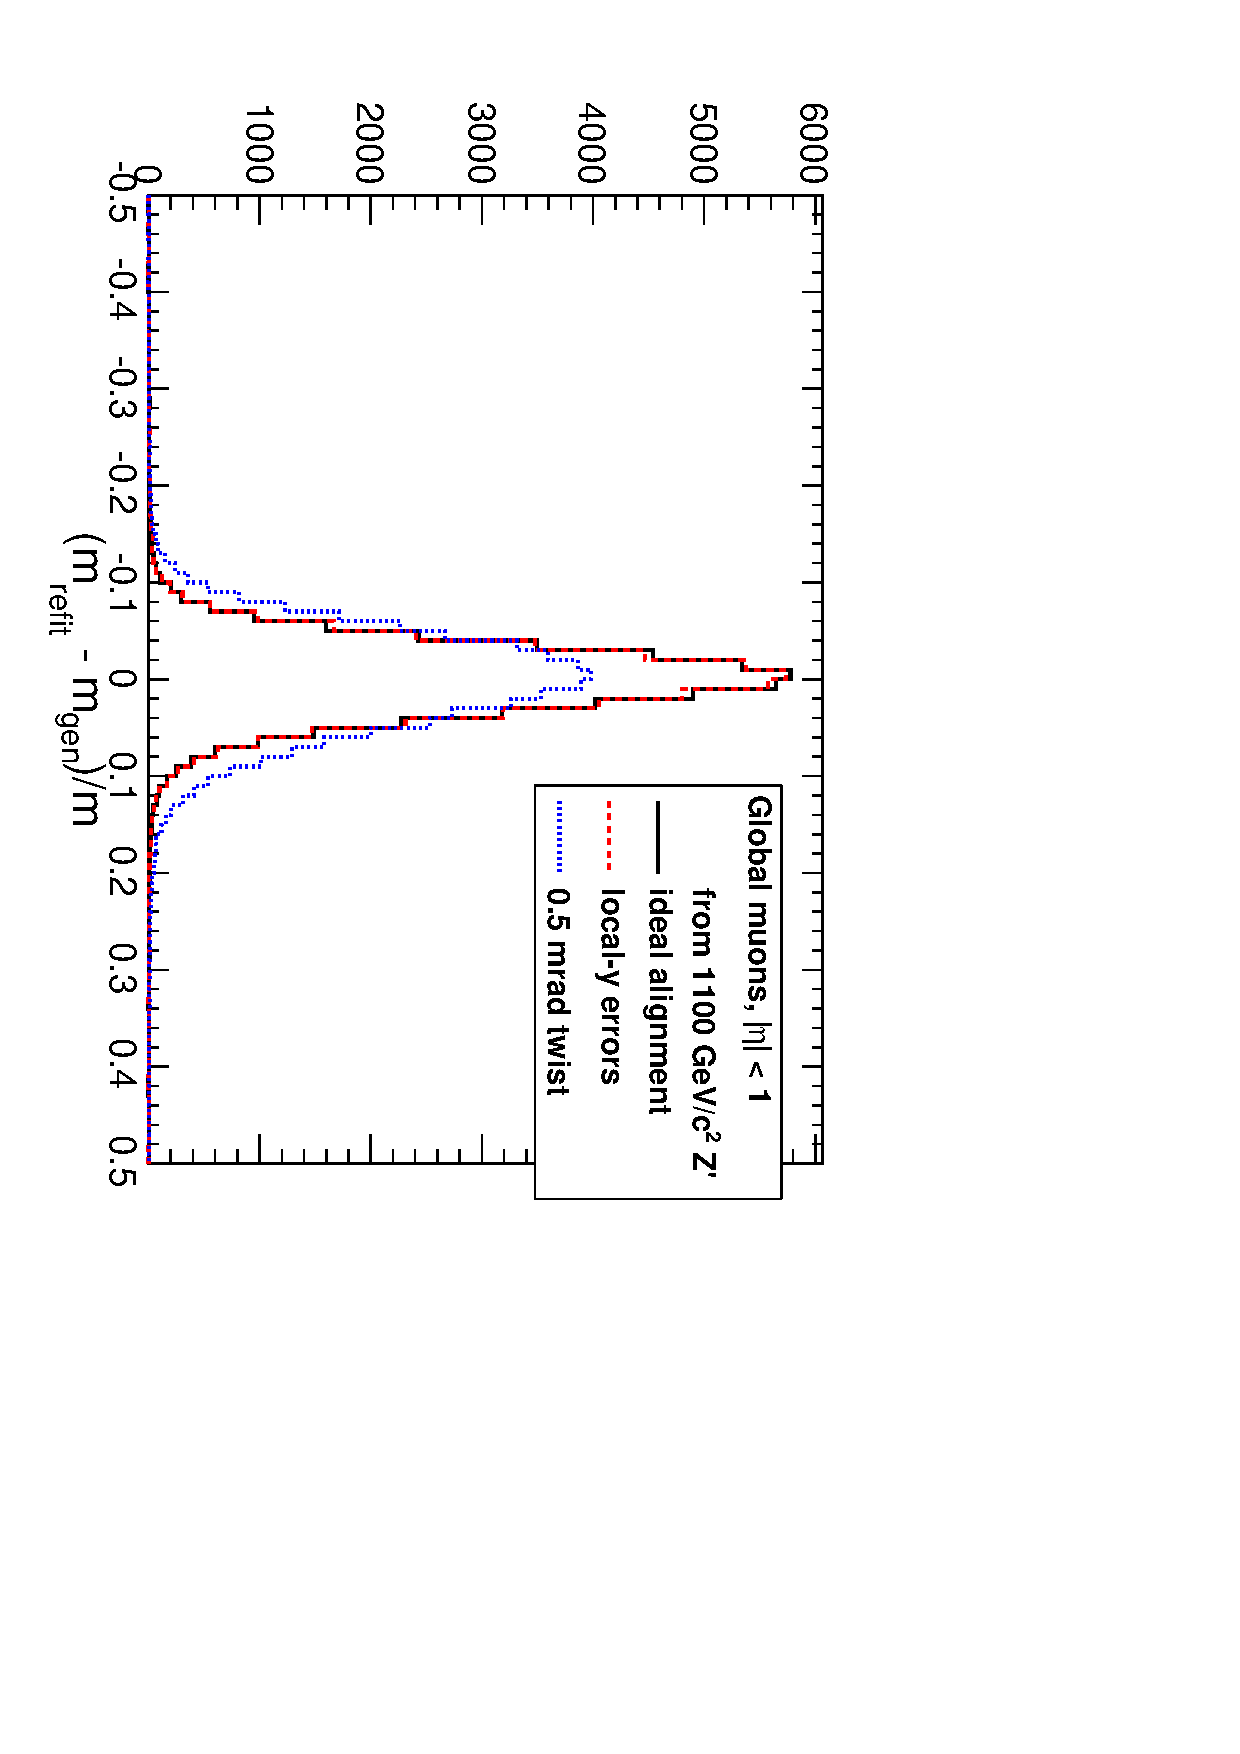
\includegraphics[height=0.65\linewidth, angle=90]{massdistribution_1100_GlobalMuons2.pdf}

\end{itemize}
\end{columns}
\end{frame}

\begin{frame}
\frametitle{Resolving the twist}
\begin{itemize}
\item Follow-up tests (pattern of residuals, cross-check with inclinometers) were performed, but they didn't isolate the problem and lead to a diagnosis

\hfill 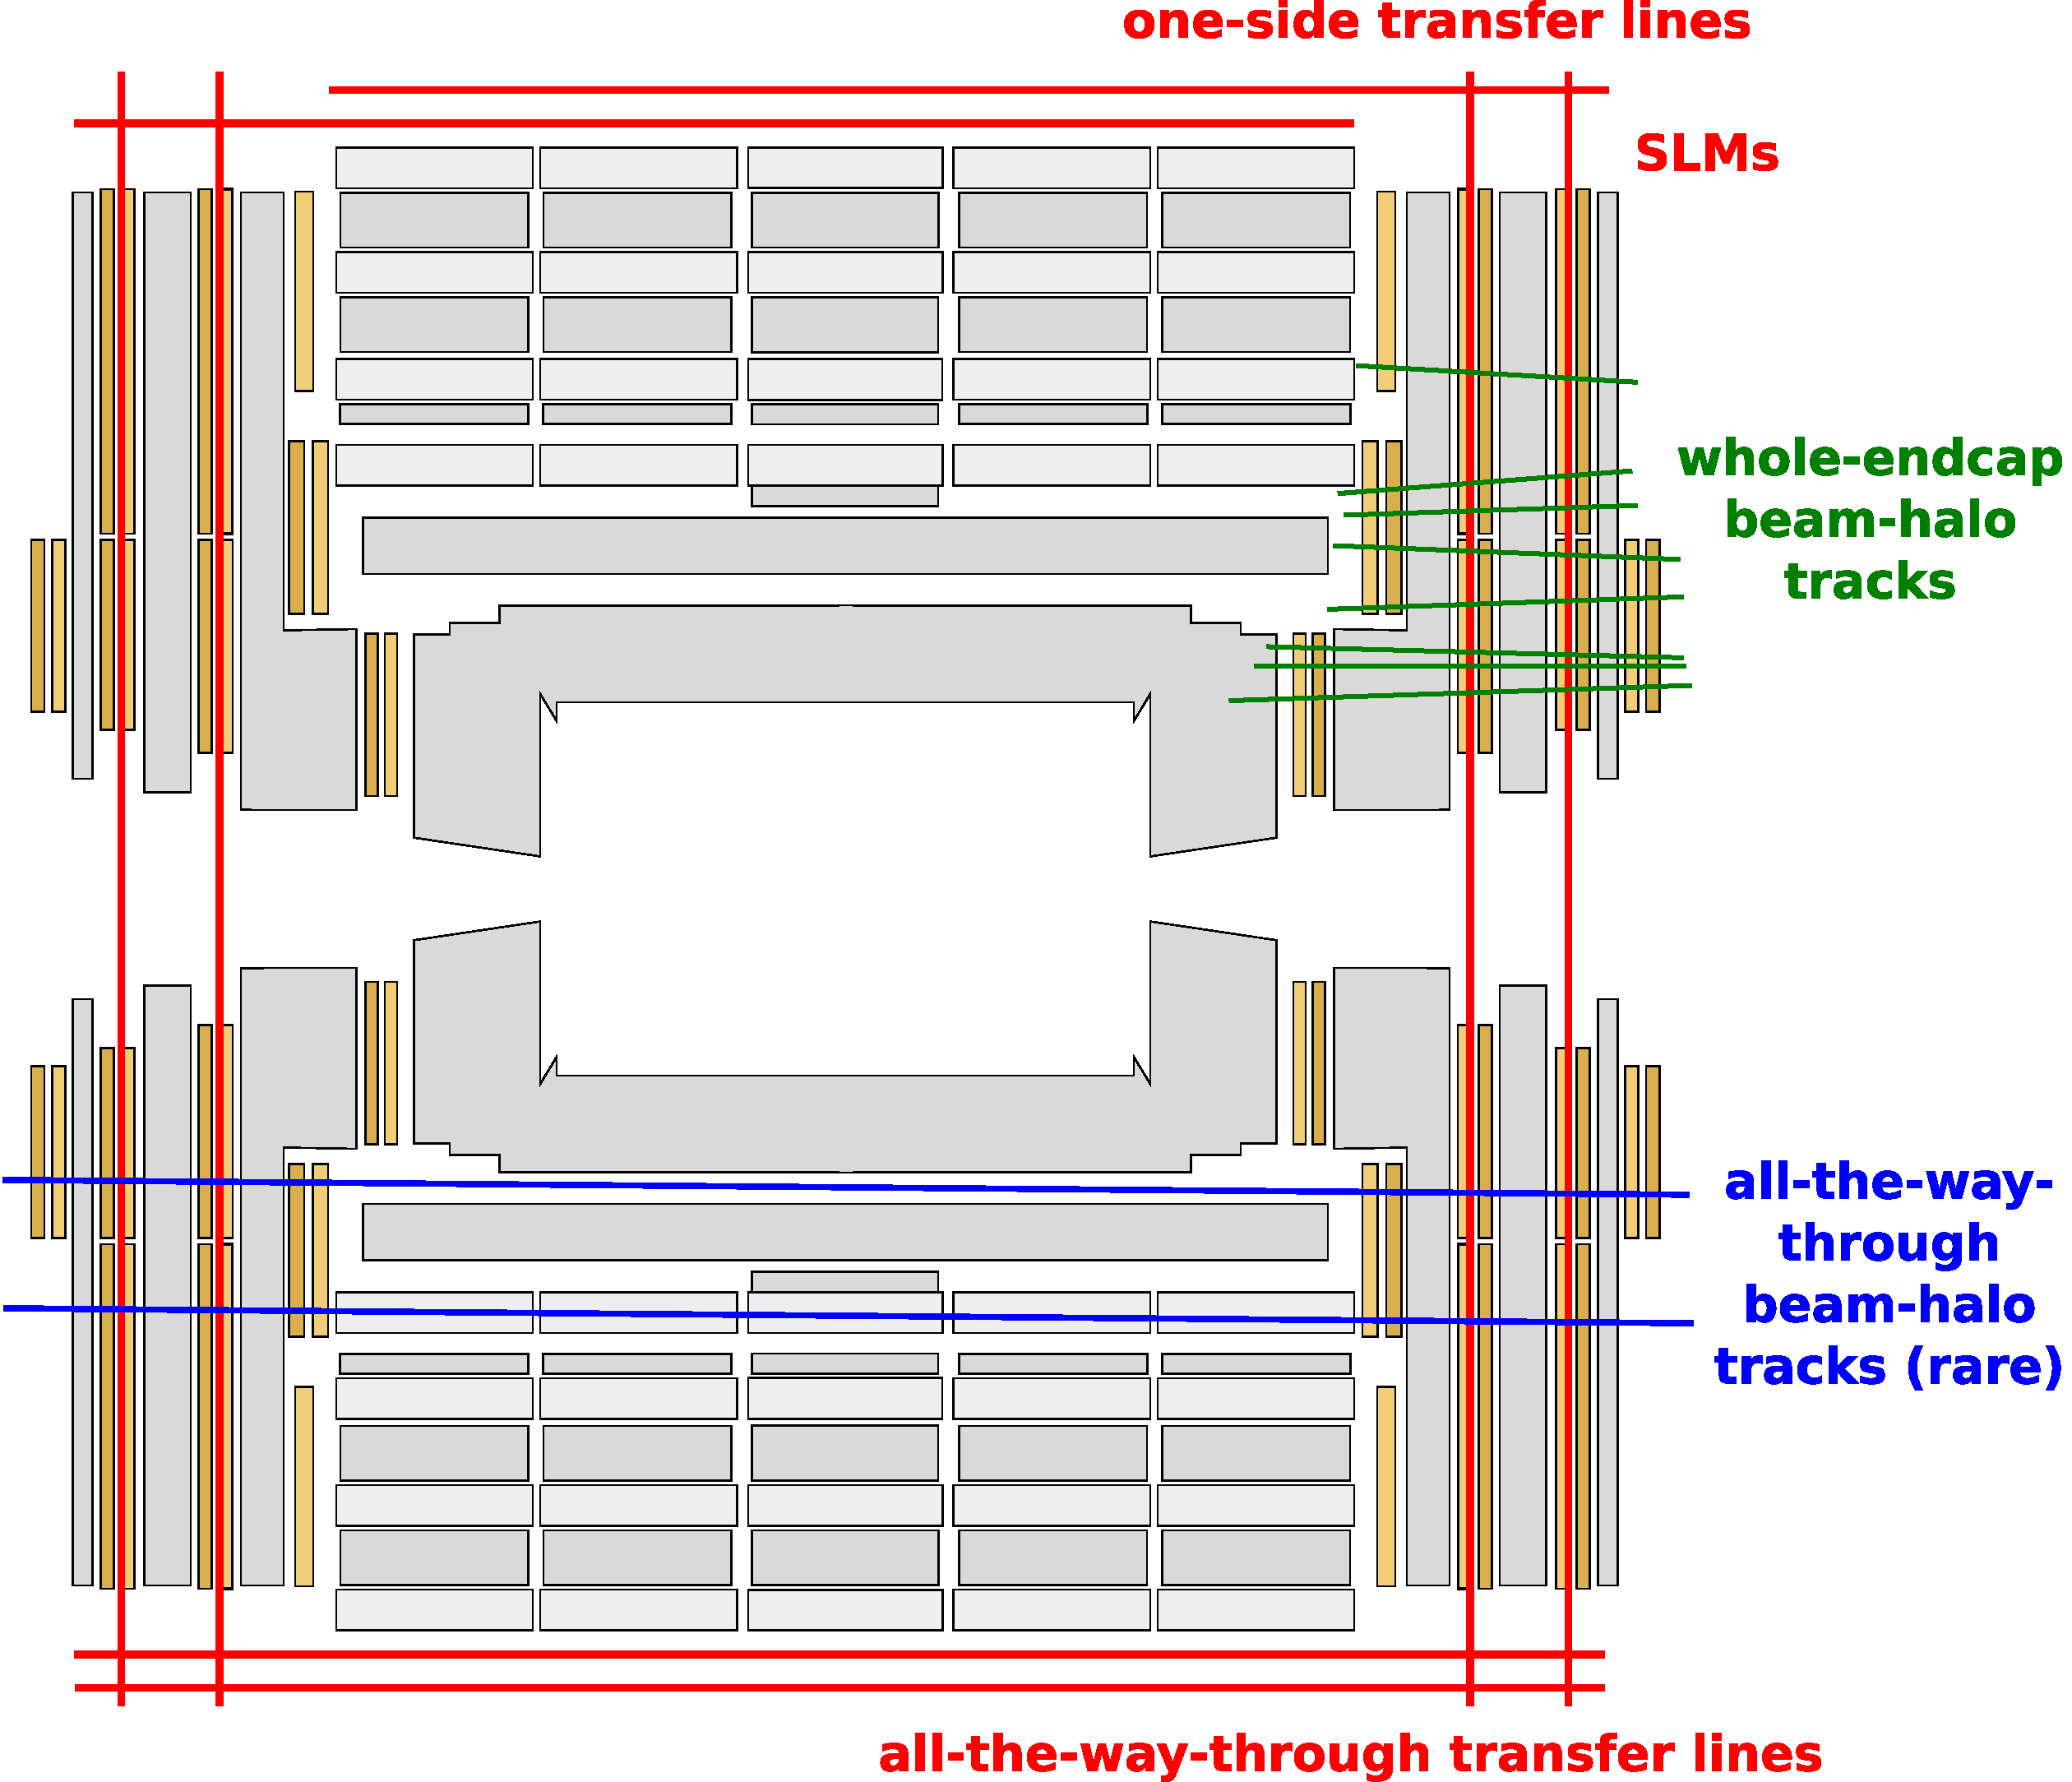
\includegraphics[width=0.6\linewidth]{beamhalo_transferlines.pdf}

\vspace{-5.3 cm}
\item More decisive test:
\begin{enumerate}\setlength{\itemsep}{0.2 cm}
\item align endcap disks \\ with beam-halo \\ (instead of global \\ muons from tracker)
\item use SLM/transfer \\ lines to propagate \\ measurement to \\ the barrel (instead of \\ an independent fit)
\item check for barrel twist \\ relative to transfer lines, which are fixed by endcap tracks
\end{enumerate}

\item CSC beam-halo tracks are very unlikely to have a twist of their own with the same magnitude as tracker-to-DT GlobalMuons
\end{itemize}
\end{frame}

\begin{frame}
\frametitle{Resolving the twist}
\begin{itemize}
\item This new test would provide a tighter network of cross-checks, with
  track-based checks between hardware steps and vice-versa

\item When there is a discrepancy at some step (and there must be one), it
  will isolate the problem, hopefully leading to a solution
\end{itemize}

\vfill
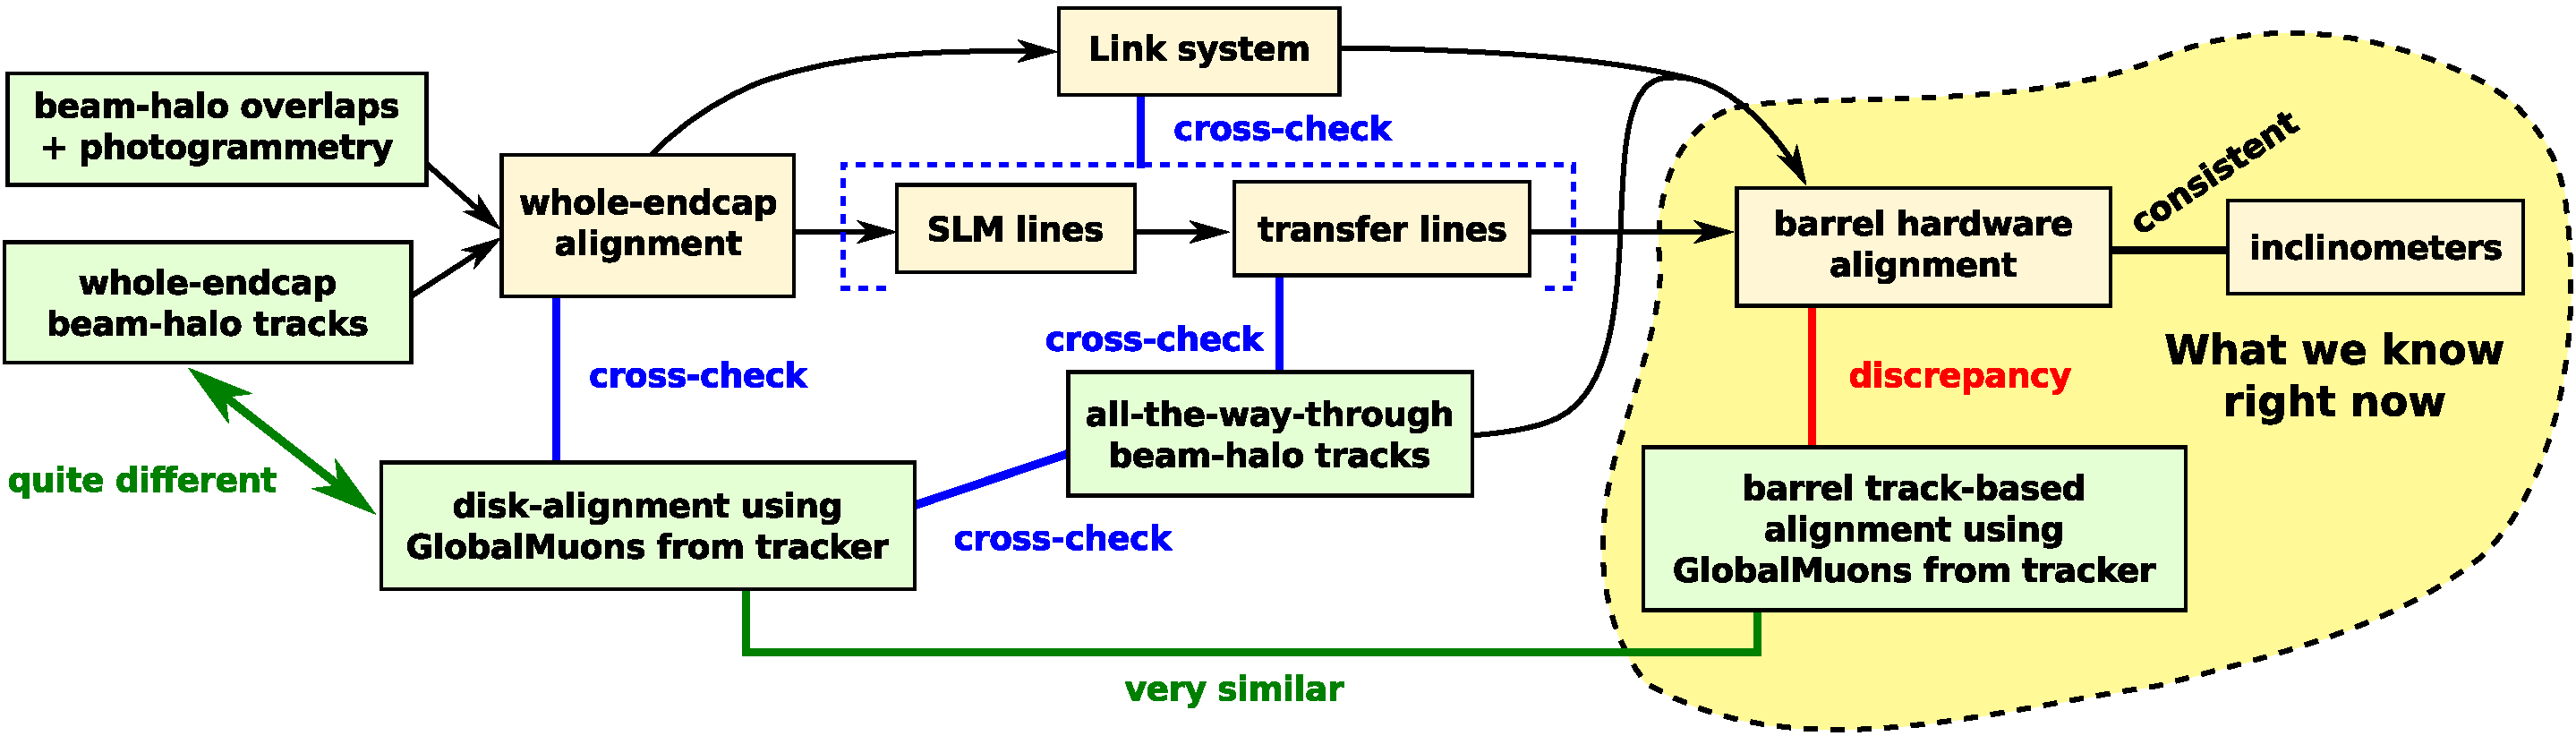
\includegraphics[width=\linewidth]{together.pdf}

\vfill
\begin{itemize}
\item Incidentally, this brings all hardware alignment systems and all
  track-based techniques into a single round of comparisons
\end{itemize}
\end{frame}

%% \section*{First section}
%% \begin{frame}
%% \begin{center}
%% \Huge \textcolor{blue}{First section}
%% \end{center}
%% \end{frame}

\begin{frame}
\frametitle{New constants for re-reco}
\begin{itemize}
\item Schedule of the next sign-off:
\begin{enumerate}
\item Friday, Oct $N$ ($N = 15$?): finalized alignment {\it procedures}, decision about track-based vs.\ hardware in barrel
\item same day: tracker alignment is frozen
\item following week: re-align with new tracker geometry
\item next Friday: finalized {\it constants} (no discussion about procedures or track-based vs.\ hardware)
\item constants passed on to Muon POG for testing\ldots
\end{enumerate}

\item Targeted for next sign-off:
\begin{itemize}
\item \textcolor{darkblue}{barrel track-based} with understood/controlled residuals-inside- of-chambers, possibly lower $p_T$ cut in cosmics
\item \textcolor{darkblue}{barrel hardware} with all-at-once fit
\item \textcolor{darkblue}{endcap disk} with lower $p_T$ cut, possibly using collisions muons
\item \textcolor{darkblue}{endcap hardware} improvements in $z$ of chambers/disks
\item endcap beam-halo $\to$ transfer lines $\to$ barrel method to resolve track-based vs.\ hardware twist issue
\end{itemize}
\end{itemize}
\end{frame}

\begin{frame}
\frametitle{Conclusions}
\begin{itemize}\setlength{\itemsep}{0.25 cm}
\item Track-based alignment with 20--30~pb$^{-1}$ of collisions muons
  is marginal; best track-based alignment still from cosmics
\item Continuing to study systematic errors with cosmics
\item Improvement to endcap disk alignment is in development
\item We may be able to resolve the ``twist'' issue by using all
  alignment subsystems (barrel, endcap, link), and tracks from
  different sources (tracker-to-muon chambers, endcap beam-halo)
\item Several improvements targeted for next reprocessing
\end{itemize}
\label{numpages}
\end{frame}

\end{document}
